% =============================================================
\section{Implications and Applications of the Compton Formula}
% =============================================================

The Compton formula is given by
\[
\Delta \lambda = \lambda' - \lambda = \frac{h}{m_e c}(1 - \cos\theta)
\]

\begin{PhysicsBox}[Physical Meaning]
	The Compton formula describes the increase in wavelength \(\Delta \lambda\)
	of a photon after elastic scattering by an electron.
	The shift depends only on the scattering angle \(\theta\) —
	not on the energy of the incident photon.
\end{PhysicsBox}


\subsection*{Maximum Compton Shift}

The maximum value occurs for \( \theta = 180^\circ \), since \( 1 - \cos(180^\circ) = 2 \). Thus,

\begin{align*}
	\Delta \lambda_\text{max} &= 2 \cdot \frac{h}{m_e c}
	= 2 \cdot \frac{6.626 \times 10^{-34}~\text{Js}}{9.109 \times 10^{-31}~\text{kg} \cdot 3.0 \times 10^8~\text{m/s}}\\
	&= 4.85 \times 10^{-12}~\text{m}
\end{align*}


\begin{DidacticBox}[The Compton Wavelength Factor]
	The quantity
	\[
	\lambda_C = \frac{h}{m_e c} = 2.43 \times 10^{-12}~\text{m}
	\]
	is called the \emph{Compton wavelength of the electron}.
	It is a fundamental constant of nature that indicates
	how strongly photons change their wavelength in maximum backscattering (\(\theta = 180^\circ\)).
\end{DidacticBox}


\subsection*{Comparison for Different Radiation Types}

This wavelength shift can now be compared with typical photon wavelengths:

\begin{center}
	\begin{tabular}{|l|c|c|c|}
		\hline
		\textbf{Type of radiation} & \(\lambda\) [m] & \(\Delta \lambda\) [m] & \(\frac{\Delta \lambda}{\lambda}\) \\
		\hline
		Red light & \(7.0 \times 10^{-7}\) & \(4.85 \times 10^{-12}\) & \(6.93 \times 10^{-6}\) \\
		X-rays & \(1.0 \times 10^{-11}\) & \(4.85 \times 10^{-12}\) & \(0.485\) \\
		Gamma rays & \(1.0 \times 10^{-13}\) & \(4.85 \times 10^{-12}\) & \(48.5\) \\
		\hline
	\end{tabular}
\end{center}

\begin{NoteBox}[Comparison with the Visible Range]
	For visible light (\(\lambda \approx 700\,\text{nm}\)), 
	the relative change \(\Delta \lambda / \lambda\) is negligibly small,
	while it becomes clearly measurable for X-rays and gamma radiation.
\end{NoteBox}


\subsection*{Conclusion}

\begin{itemize}
	\item For visible light (e.g. \( \lambda = 700\,\text{nm} \)), the Compton shift is practically unmeasurable.
	\item In the X-ray range, \(\Delta \lambda\) is comparable to \(\lambda\); the effect is clearly observable experimentally.
	\item For gamma rays, \(\Delta \lambda\) exceeds the original wavelength by far.
\end{itemize}

\begin{PhysicsBox}[Why X-rays?]
	The Compton effect was discovered in 1923 using X-rays,
	because only in this energy range is the wavelength shift large enough to be measurable.
	For visible light, the effect would be many orders of magnitude too small.
\end{PhysicsBox}

\newpage
\noindent

\subsection*{Relative Compton Shift as a Function of Wavelength}

\begin{figure}[h]
	\centering
	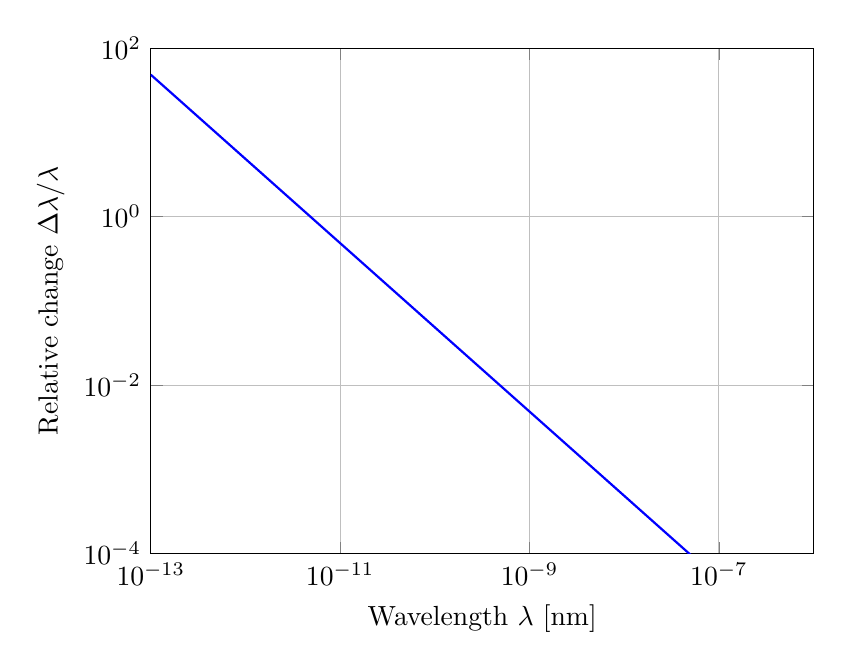
\begin{tikzpicture}
		\begin{axis}[
			width=10cm,
			height=8cm,
			xlabel={Wavelength $\lambda$ [nm]},
			ylabel={Relative change $\Delta \lambda / \lambda$},
			xmode=log,
			ymode=log,
			grid=both,
			minor grid style={gray!20},
			major grid style={gray!50},
			domain=1e-13:1e-6,
			samples=500,
			xmin=1e-13, xmax=1e-6,
			ymin=1e-4, ymax=1e2,
			xtick={1e-13,1e-11,1e-9,1e-7},
			xticklabels={$10^{-13}$, $10^{-11}$, $10^{-9}$, $10^{-7}$},
			ytickten={-4,-2,0,2}
			]
			\addplot [
			thick,
			blue
			]
			expression {
				4.849416e-12 / x
			};
		\end{axis}
	\end{tikzpicture}
	\caption{Relative wavelength change $\Delta \lambda / \lambda$ according to the Compton formula for $\theta = 180^\circ$ as a function of the incident wavelength $\lambda$.}
\end{figure}
